In this appendix the reader will be presented with a brief mathematics discussion regarding some common \acrshort{cv} models and problems, which could be useful to better understand what is discussed in chapter \ref{chap:third-chapter}.

\section{Pinhole Camera Model}\label{subsection:pinhole}
The pinhole camera model is camera model which is widely used in \acrfull{cv}. Despite being a relatively simple model, it is still accurate enough for the vast majority of applications. The pinhole camera model is used to describe the mathematical relationship which exists between the coordinates of a point in the \acrshort{3d} world and its projection onto the image plane. In the pinhole camera model, the light passes trough a single point, the camera center, before being projected onto the image plane, and no lenses are used to focus light, so geometrical distortions or blurring are not modeled in the pinhole camera model.

\begin{figure}[htbp]
  \centering
  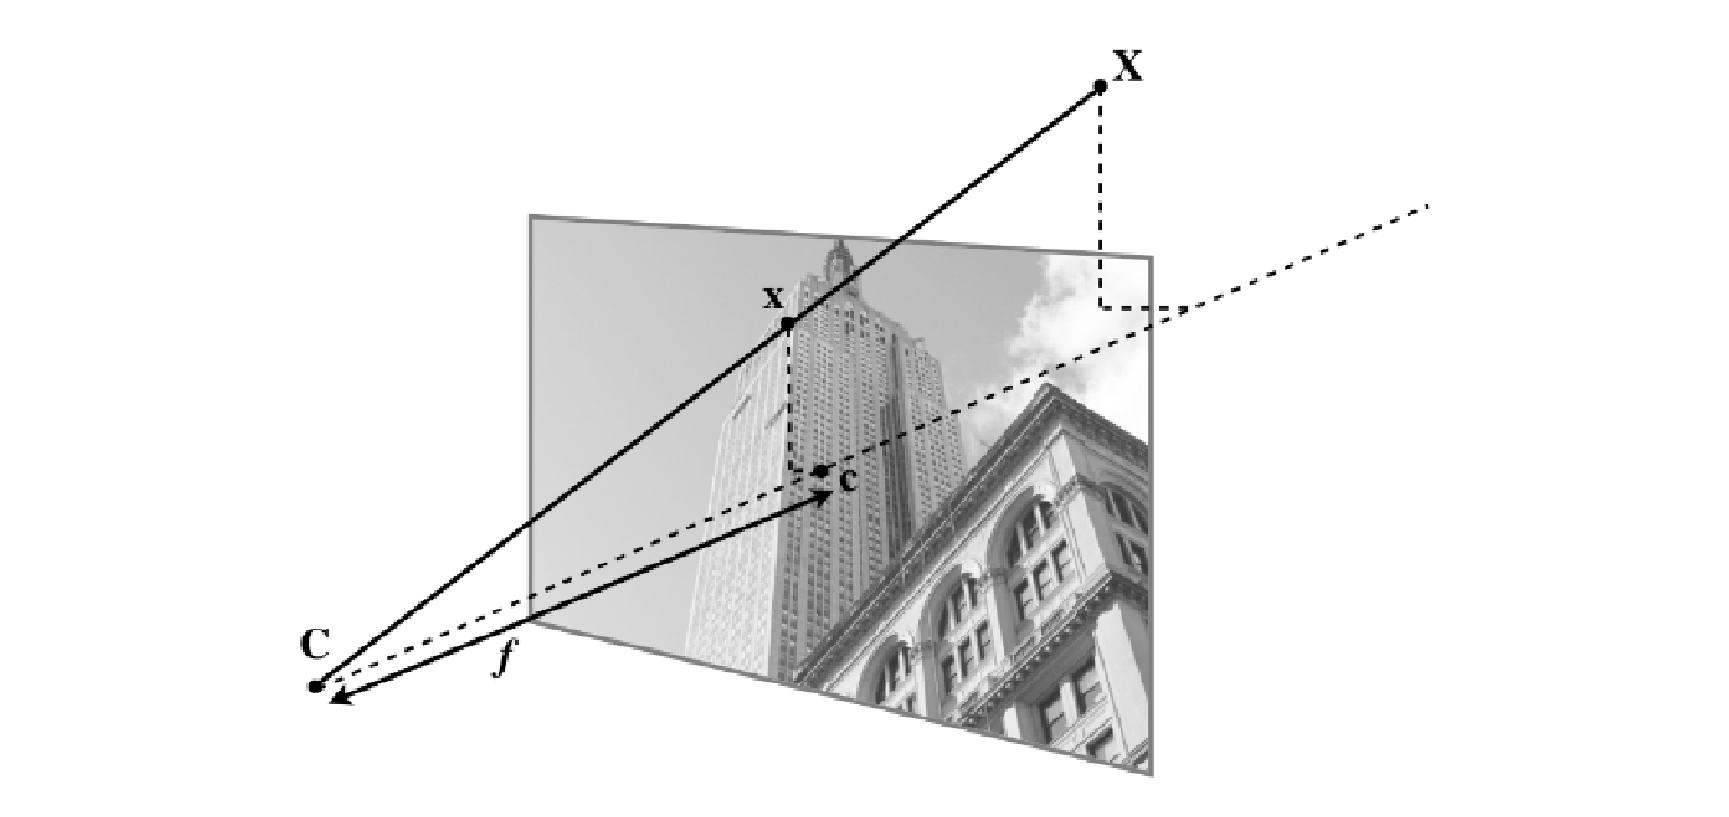
\includegraphics[width=0.85\textwidth]{gfx/pinholeCamera.eps}
  \caption{The pin-hole camera model \cite{solem2012programming}}
  \label{fig:pinholeCamera}
\end{figure}

By referring to \ref{fig:pinholeCamera}, a \acrshort{3d} point $\mathbf{X}$ is projected to an image point $\mathbf{x}$ (both expressed in homogeneous coordinates) as :

\begin{equation*}
  \lambda\mathbf{x}=P\mathbf{X} \,,
\end{equation*}

where $P$ is a 3-by-4 matrix called camera matrix and $\lambda$ is a scalar number representing the inverse depth of the \acrshort{3d} point. As a result, the \acrshort{3d} point $\mathbf{X}$ is characterized by four elements, $X = [X, Y , Z, W ]$ in homogeneous coordinates.
Generally, the camera matrix $P$ can be decomposed as :

\begin{equation*}
  P = K[R \ | \ \mathbf{t}] \,,
\end{equation*}

where $R$ is the rotation matrix which describes the orientation of the camera, $\mathbf{t}$ is a \acrshort{3d} translation vector which describes the position of the camera center and $K$ is the intrinsic camera calibration matrix.
The camera calibration matrix basically describes the projection properties of the camera and can be written as :

\begin{equation*}
  K = \begin{bmatrix}
    \alpha f & s & c_x \\
    0        & f & c_y \\
    0        & 0 & 1
  \end{bmatrix} \,,
\end{equation*}

where $\alpha$ is the aspect ratio of the sensor's pixels, $f$ is the focal length, $s$ is the skew and $c_x$, $c_y$ are the coordinates of the optical center (or also called the principal point) of the image. Usually the principal point of the image can be approximated with half the height and half the width of the image. The skew is used only if the pixel array in the sensor is skewed. In most cases is safe to assume $s = 0$.
By defining :

\begin{equation*}
  f_x = \alpha f_y
\end{equation*}

and by neglecting $s$ we can write the calibration matrix in the most common form :

\begin{equation*}
  K = \begin{bmatrix}
    f_x & 0   & c_x \\
    0   & f_y & c_y \\
    0   & 0   & 1
  \end{bmatrix} \,,
\end{equation*}

If we make the assumption of square pixel, then $\alpha = 1 $ and $ f_x = f_y = f$, and so we can write the camera calibration matrix as :

\begin{equation*}
  K = \begin{bmatrix}
    f & 0 & c_x \\
    0 & f & c_y \\
    0 & 0 & 1
  \end{bmatrix} \,.
\end{equation*}

More information about camera model and camera calibration matrix can be found in \cite{10.5555/861369} and \cite{Pollefeys2004}.

\section{Image Derivatives}\label{sec:imagegradient}
For a grayscale image, the image intensity changes over the image itself can be described by using the $x$ and $y$ derivatives, $I_x$ and $I_y$ of the graylevel image $I$.
Once defined the image derivatives, it is possible to define another quantity, the image gradient, which is the vector:

\begin{equation*}
  |\nabla I| = \sqrt{I_x^2 + I_y^2} \,,
\end{equation*}

which describes how strong the image intensity change. Image derivatives can be computed using a discrete approximations, which are implemented as convolutions:

\begin{equation*}
  I_x = I * D_x \ \ \,, \ \ I_y = I * D_y \,,
\end{equation*}

where $D_x$, $D_y$ are the kernel of the derivative and $*$ is the \acrshort{2d} convolutional operation. Two common choices for $D_x$, $D_y$ are either the so called Prewitt filters :

\begin{equation*}
  D_x = \begin{bmatrix}
    -1 & 0 & 1 \\
    -1 & 0 & 1 \\
    -1 & 0 & 1
  \end{bmatrix} \ \ \,,  \ \
  D_y = \begin{bmatrix}
    -1 & -1 & -1 \\
    0  & 0  & 0  \\
    1  & 1  & 1
  \end{bmatrix}\,,
\end{equation*}

or the so called Sobel filters:

\begin{equation*}
  D_x = \begin{bmatrix}
    -1 & 0 & 1 \\
    -2 & 0 & 2 \\
    -1 & 0 & 1
  \end{bmatrix} \ \ \,,  \ \
  D_y = \begin{bmatrix}
    -1 & -2 & -1 \\
    0  & 0  & 0  \\
    1  & 2  & 1
  \end{bmatrix}\,,
\end{equation*}

\section{The Hough Transform}\label{sec:hough}
The Hough transform is a method often used in \acrshort{cv} for finding shapes in images. It works by using a voting procedure in the parameters space of the shapes. The most common use of the Hough transform is to find lines in images.
Consider the straight line equation, in its polar form,

\begin{equation*}
  \rho = x \cos{\theta} + y \sin{\theta} \,,
\end{equation*}

\begin{figure}[htbp]
  \centering
  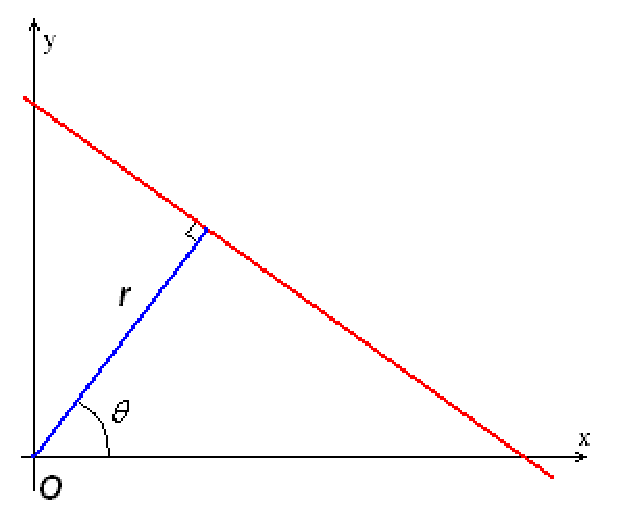
\includegraphics[width=0.45\textwidth]{gfx/R_theta_line.eps}
  \caption{Polar representation of a straight line \cite{pichough}}
  \label{fig:linePolar}
\end{figure}

where $\rho$ obviously is the distance from the origin of the reference system to the closest point on the straight line, while $\theta$ is the angle between the x axis and the line connecting the origin with that closest point.
The linear Hough transform algorithm estimates the two parameters that define the straight line. The transform space has two dimensions, and any point in the transform space is used as an accumulator (a bi-dimensional vector) to detect a line described by the aforementioned polar equation of the straight line. Every point in the detected edges in the image contributes to the accumulators. Generally, the dimension of the accumulator is equal to the number of unknown parameters, which in this case are two, $\rho$ and $\theta$. For each pixel and is neighborhood, the algorithm which computes the Hough transform first try to detect if the specific pixel which is being analyzed lie on a line. If so, computes $\rho$ and $\theta$ of that line, and then look for the accumulator's bin that the parameters fall into, and increment the value of that bin.
By searching the boxes with highest values, typically by looking at local maxima in the accumulator space, it is possible to identify the the most likely lines. The final result of the Hough transform will be a \acrshort{2d} matrix, were one dimension will be represented by $\theta$ and the other one by $\rho$.
Each element of that matrix will have a value equal to the sum of the pixels that are positioned on the line represented by the parameters $\rho$, $\theta$. So the element with the highest value indicates the straight line that is most represented in the input image \cite{houghreport}. More information about the how the Hough transform works can be retrieved in \cite{10.1145/361237.361242} and \cite{osti_4746348}.

\section{Perspective-n-Point Problem}
The \acrfull{pnp} point is the problem of determining the position and the orientation of a calibrated camera given its intrinsic parameters and a set of correspondences between a given set of \acrshort{3d} points and their respective \acrshort{2d} projections in the image \cite{10.1007/s11263-008-0152-6}.
The perspective projection for a standard pinhole camera that has been introduced in section \ref{subsection:pinhole} leads to the following equation (in homogeneous coordinates) for the model:

\begin{equation*}
  \lambda
  \begin{bmatrix}
    u \\
    v \\
    1 \\
  \end{bmatrix}
  =
  \begin{bmatrix}
    f & 0 & c_x \\
    0 & f & c_y \\
    0 & 0 & 1
  \end{bmatrix}
  \begin{bmatrix}
    r_{11} & r_{12} & r_{13} & t_1 \\
    r_{21} & r_{22} & r_{23} & t_2 \\
    r_{31} & r_{32} & r_{33} & t_3
  \end{bmatrix}
  \begin{bmatrix}
    x \\
    y \\
    z \\
    1 \\
  \end{bmatrix} \,,
\end{equation*}

were $r_{ij}$ and $t_i$ are the components of the rotation matrix and the translation vector which are being calculated, respectively.
Several methods exists for solving the \acrshort{pnp} problem, the two most common of which are the P3P method and the \textit{e}\acrshort{pnp} method. More information about their implementations can be found on  \cite{XiaoShanGao2003} \cite{Torr2000} and \cite{10.1007/s11263-008-0152-6}.
